\documentclass[8pt, a4paper]{article}
\usepackage{geometry}
\geometry{total={170mm, 257mm},left=20mm, top=20mm}
\usepackage{graphicx}


\begin{document}
\setlength \topmargin{-1in}
\title{\textbf{Software Engineering for Distributed and Interactive Systems.}}
\author{\textbf{James Ravenhill}}
\date{}
\maketitle

\section{Introduction} 

The main outcome at the beginning of the project was to create a simple and easy to used piece of software which allows the user to control the buggy without being too complex. Both the hardware and software have been an ongoing development based on feedback given through multiple tests, which a few friends generously took part in. The main objectives of the project are listed below but not limited to:

\begin{itemize}
	\item Reliability - Unreliable connection/data transfer is a disadvantage and creates more problems. This will be explained later in more detail.  
	\item  Multiple methods of communication - By using WiFi, Bluetooth, IR remote and PC. 
	\item Scalability - There should be no software problems while developing the increased load of sensor/capabilities of the buggy. 
	\item
\end{itemize}


\section{Design}
\begin{figure}[h]
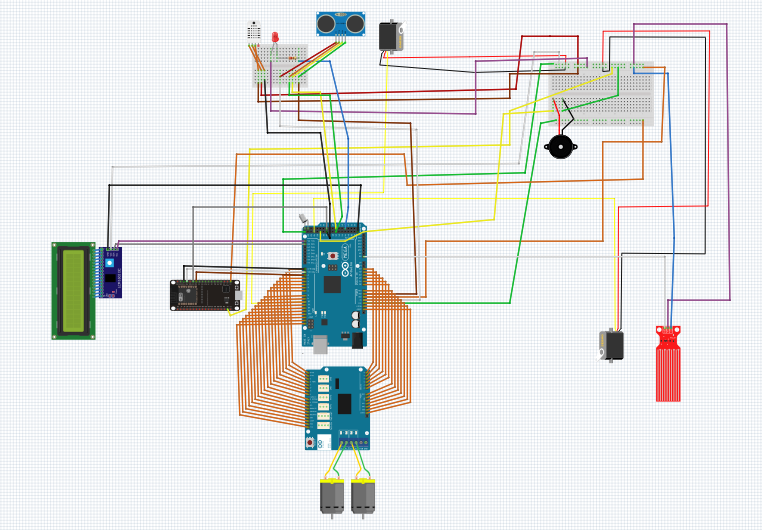
\includegraphics[height=5cm, width=7.5cm]{schematic}
\centering
\end{figure}

////TCP- Reliable, Flow control(wont overwhelm reciever), congestion control. Breaks info into packets
///UDP- unreliable,, no flow control, no congestion control

///Layers- layered system to allow for easy maintenance, ease of updating/developing the system. ADD A DIAGRAM OF THE LAYERS HERE. 

\section{Implementation}


\section{Testing}

\section{Evaluation}


\section{Code quality/remarks} ////this may get cut if needed as in more an non written task
////discuss multi and single core methods in a ReadMe file!!!


\section{Demonstration}
////film the video and then refer to it for the following subsections


\subsection{Distribution}
///Define what a distributed system is 

\subsection{Interactive}
///Define what an interactive system is

\subsection{Performance}






\section{Conclusion}


\section{Reference Library and appendices}




\end{document}